\scanpage{6}

% Reused typescript strip, running from the bottom toward the top at left.
\[
\underline{\mathrm B}=(\text{Gr-stacks})\qquad
\widehat{\underline{\mathrm B}}\qquad
\underline{\mathrm B}(\unsure{0|\mathrm O})^{\wedge}
\]
commutes not only with arbitrary projective limits, but equally with arbitrary direct limits, or what amountsto the same, that direct limits in the category (Gr-stacks) can be computed component-wise. (Here \(\underline{\mathrm B}(0)\) stands for the full subcategory of \(\underline{\mathrm B}\) formed by the basic objects \(\underline{\mathrm D}_n\), \(n\ \underline{\mathrm N}\) .)

% Handwritten notes on the reused sheet. The repeated typewriter 0 follows the
% first local 0/O alternative above; the typeface alone does not resolve it.
\handwritten{
\[
\widetilde{\mathbb D}\qquad
\unsure{N|\mathscr N}\longmapsto
\overset{\deleted{\unsure{I_n|D_n}}}{\widetilde D_n}
\]

\[
\begin{aligned}
&1+n\mathbin{.}2^1+\frac{n(n-1)}{2}\,2^2\ \text{---}\ +2^n\\
&\qquad=(1+2)^n=
\end{aligned}
\]

\diagram{\begin{tikzcd}[ampersand replacement=\&,row sep=1.15em,column sep=2em]
\widetilde D_{n'}\arrow[r,bend left=38]\arrow[r]\arrow[r,bend right=38]\&
\widetilde D_n\\
\&\widetilde D_n\arrow[d]\\
\&n\in\mathbb I
\end{tikzcd}}
\[
\begin{aligned}
d_n\in\widetilde D_n&\longrightarrow\deleted{N}\mathbb I
 &\qquad d_n&\longmapsto n\\
&\text{strictement}\\
&\text{croissante}\\
&\text{image \unsure{est|\(\subset\)}}\ \mathbb I_{\deleted{\unsure{\in n}}\leq n}
\end{aligned}
\]

% Two detached short pen traces between the upper diagrams and the prose;
% their function is not determined.
\figure{\begin{tikzpicture}[line width=.5pt,line cap=round]
\draw (0,0)--(.13,-.005);
\fill (2.62,-1.15) circle[radius=.018];
\draw (2.68,-1.23)..controls(2.78,-1.21)and(2.91,-1.25)..(3.02,-1.25);
\end{tikzpicture}}

% margin note written sideways; rotate the source 90 degrees counterclockwise.
% Both membership arches open downward in this readable orientation.
% The eta/y and xi/f/x alternatives are marked at their first live occurrence;
% subsequent occurrences use the first candidate, without settling the alphabet.
\margin{\resizebox{.99\marginparwidth}{!}{\begin{minipage}{17em}
\diagram{\begin{tikzcd}[ampersand replacement=\&,column sep=1.3em,row sep=.65em]
J_{n''}\arrow[r,"{\unsure{u_\eta|u_y}}"] \&
 {\overset{\substack{\eta\\\rotatebox{-90}{\(\in\)}}}{J}_{n'}}
 \arrow[r,"{\overset{\deleted{\unsure{u_\eta|u_g}}}{\unsure{u_\xi|u_f|u_x}}}"]
 \arrow[dr,bend right=16,sloped,"\unsure{u}"'] \&
 {\overset{\substack{\xi\\\rotatebox{-90}{\(\in\)}}}{J}_{\deleted{\unsure{n'}}n}}\\
 \& \& \xi
\end{tikzcd}}
\(u_\xi u_\eta=\)
\end{minipage}}}

\[
\widetilde D_{n'}\longrightarrow\widetilde D_n
\]
% The one live D_n lies between the two membership levels.
\diagram{\begin{tikzcd}[ampersand replacement=\&,column sep=1.25em,row sep=.8em]
x''\arrow[d,dash,"\deleted{\unsure{I|=}}"'] \& {<} \&
x'\arrow[d,dash]\arrow[d,phantom,"\cdot"'] \& {\in} \&
|[yshift=-.6em]|{\overset{\deleted{D}}{\widetilde D_n}}\\
y'' \& {<} \& y'\arrow[d,dash] \& {\in} \& {}\\
n'' \& \& n' \& \&
\end{tikzcd}}
% The small dot beside the right connector is a literal detached mark.
\figure{\begin{tikzpicture}[line width=.6pt]
\draw (0,.75)..controls(.8,.52)and(.7,-.3)..(1.25,-.48)
 (.03,.32)..controls(.48,.08)and(.37,-.5)..(1.04,-.64);
\fill (2.7,-.48) circle[radius=.04] (2.7,-.88) circle[radius=.04];
\end{tikzpicture}}

\(I\) ens ordonné

\(n\longmapsto\widetilde D_n\) famille d'ens ordonnés \unsure{,|;}

\[
\widetilde D_n\xrightarrow{\deleted{\phi}\unsure{k_n|\kappa_n|K_n}}I\qquad
\text{str. croiss.}\quad\text{image}\quad I_{\leq n}
\]

Si \(n'\leq n\), \deleted{\unsure{Soit|Sinon} l'ens \(K\)} Soit
\[
\begin{gathered}
\Phi_{n',n}\subset\widetilde D_n\\[-.2em]
\rotatebox{90}{\(=\)}\\[-.2em]
\bigl\{x\in\widetilde D_n\mid k_n(x)=n'\bigr\}
\end{gathered}
\]
% k_n follows the first local k/kappa/K alternative; its two arms exclude tau.

\deleted{Soit \(x\in\Phi_{n'},\)}

Considérons l'ens \deleted{\(\unsure{\widetilde D_{n'}|D_n}\)}\(\unsure{B|\mathbb B|\mathscr B}\)

\diagram{\begin{tikzcd}[ampersand replacement=\&,column sep=2.3em]
F_0 \& \mathbb F_1\arrow[l,shift left=.6ex]\arrow[l,shift right=.6ex]
 \& F_2\arrow[l,shift left=.6ex]\arrow[l,shift right=.6ex]
\end{tikzcd}}
% The loop has separate departure and return ends to the right of x;
% no extra filled vertex is supplied.
\diagram{\begin{tikzcd}[ampersand replacement=\&,column sep=1em]
x\arrow[loop right,distance=2em,in=35,out=-35] \& {}
\end{tikzcd}}
\diagram{\begin{tikzcd}[ampersand replacement=\&,row sep=1.1em]
x'\arrow[d,dash]\\ y'
\end{tikzcd}}
\figure{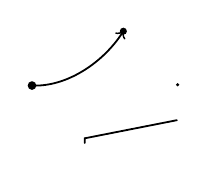
\begin{tikzpicture}[line width=.65pt,line cap=round]
\fill (0,.15) circle[radius=.055];
\draw[->] (0,.15)..controls(.45,.13)and(.91,.45)..(1.16,.84);
\fill (1.16,.84) circle[radius=.045] (1.85,.16) circle[radius=.022];
\draw (.67,-.58)--(.67,-.52)--(1.84,-.29);
\end{tikzpicture}}

% Small detached V-like pen trace to the left of the loop; not identified as a word.
\figure{\begin{tikzpicture}[line width=.5pt,line cap=round]
\draw (0,.05)--(.07,0) (.11,.005)--(.2,.04);
\end{tikzpicture}}
\[
\begin{aligned}
\pi_0(F_*,x)&=\text{ens des classes d'hom.topie. des}\\
&\phantom{=}\text{lacets en }x
\end{aligned}
\]
}
% archive sheet number: 5
